\documentclass[hyperref={pdfpagemode=FullScreen, colorlinks=false}]{beamer}

\usepackage{selinput}			% Inputencoding
	\SelectInputMappings{adieresis={ä}, germandbls={ß}, Euro={€}}
\usepackage[T1]{fontenc}		% Fontencoding
%
\usepackage{pifont}
\usepackage{csquotes,siunitx}			% Anführungszeichen; wird von biblatex gewünscht
\usepackage[backend=biber,citestyle=alphabetic,uniquelist=false]{biblatex}	% Literatur formatieren
\addbibresource{bodendynamik.bib}	% Literaturdatenbank
\usepackage{caption} 
\usepackage{subfig}
\usepackage{comment}
%%%%%%%%%%%%%%%%%%%%%%%%%%%%%%%%%%%%%%%%%%%%%%%%%%%%%%%%%%%%%%%%%%%%%%%%%%%%%%%%%%%%%%%%%%%%%%%%%%%%%%%
% Thema für Präsentation
\usetheme[fusszeile=ernstcolor,sprache=ngerman,seite=letzte,
verhaeltnis=16:10,
hausschrift=false,
navigation=false,
titelseite=blau]{TUBAF}

\TUBAFZweitlogo{\includegraphics{fig_pdf/UFZ_logo_inv.pdf}}

%%%%%%%%%%%%%%%%%%%%%%%%%%%%%%%%%%%%%%%%%%%%%%%%%%%%%%%%%%%%%%%%%%%%%%%%%%%%%%%%%%%%%%%%%%%%%%%%%%%%%%%
% Optionen für Anmerkungen
\mode<presentation>{%
\setbeameroption{hide notes}				% keine Notizen (default)
%\setbeameroption{show notes}				% Notizen und Frames gemischt
%\setbeameroption{show only notes}			% nur Notizen
%
%\usepackage{pgfpages}					% wird für nachfolgendes benötigt
%\setbeameroption{show notes on second screen=left}	% wie gesagt; left, right, bottom, top
}




%%% DK packages and settings
\usepackage{amsmath}
\usepackage{pgfpages}
\pgfpagesuselayout{resize to}[a4paper, landscape]   % border shrink=5mm
\usepackage{siunitx}  
%\sisetup{locale = DE} 
\usepackage{tikz}
\usepackage{pgfplots}
\usepackage{animate}

\usetikzlibrary{math}
%\usetikzlibrary{datavisualization.formats.functions}
%\usetikzlibrary{datavisualization}
\usetikzlibrary{intersections}
\usepgfplotslibrary{groupplots,dateplot}
\pgfplotsset{compat=1.16}

\tikzset{
%DKspring(length) length=2...10
DKspring/.pic={
\coordinate (half_up) at (0.5*0.125*#1-0.5*0.125*2, 0.5*0.125*10-0.5*0.125*#1); %at (0.5*(#1-0.2), 0.5*(1.0-#1));
\coordinate (full_up)   at ( 0.125*#1-    0.125*2,     0.125*10-    0.125*#1);
\coordinate (full_down) at ( 0.125*#1-    0.125*2,    -0.125*10+    0.125*#1);
\draw (0, 0) -- ++(1, 0) -- ++(half_up)
    -- ++(full_down) -- ++(full_up) 
    -- ++(full_down) -- ++(full_up)
    -- ++(full_down) -- ++(full_up)
    -- ++(full_down) -- ++(half_up)
    -- ++(1, 0);
    },   
%DKdashpot(length) length=02...10    
DKdashpot/.pic={
\coordinate (upper_end) at (#1-0.5, 0.5);
\coordinate (lower_end) at (#1-0.5,-0.5);
\coordinate (upper_pos) at (#1-1, 0.5);
\coordinate (lower_pos) at (#1-1,-0.5);
\coordinate (center_pos) at (#1-1, 0.0);
\coordinate (center_end) at (#1, 0.0);
\draw (0, 0) -- ++(1, 0);
\draw (upper_end) -- (1, 0.5) -- (1, -0.5) -- (lower_end);
\draw (center_pos) -- (center_end);
\draw (upper_pos) -- (lower_pos);
    },
DKbase/.pic={
\draw[thick] (0, 1.5) -- (0, -1.5);
\foreach \y in {-1.5,-1.0,...,1.0} \draw[thin] (0, \y) -- +(-0.5, 0.5);
},
 invisible/.style={opacity=0},
  visible on/.style={alt={#1{}{invisible}}},
  alt/.code args={<#1>#2#3}{%
    \alt<#1>{\pgfkeysalso{#2}}{\pgfkeysalso{#3}} % \pgfkeysalso doesn't change the path
  }
}
\newlength\figH     % to scale tikzplotlib figures
\newlength\figW     % to scale tikzplotlib figures


\setbeamercovered{transparent}
%-----------------Custom footnote---------------
\TUBAFFzstrikttext{D. Kern \TUBAFfztrenner T. Nagel --- Vorlesung Bodendynamik --- Sommersemester 2021 }
%-----------------------------------------------

\tikzset{
%DKspring(length) length=2...10
DKspring/.pic={
\coordinate (half_up) at (0.5*0.125*#1-0.5*0.125*2, 0.5*0.125*10-0.5*0.125*#1); %at (0.5*(#1-0.2), 0.5*(1.0-#1));
\coordinate (full_up)   at ( 0.125*#1-    0.125*2,     0.125*10-    0.125*#1);
\coordinate (full_down) at ( 0.125*#1-    0.125*2,    -0.125*10+    0.125*#1);
\draw (0, 0) -- ++(1, 0) -- ++(half_up)
    -- ++(full_down) -- ++(full_up) 
    -- ++(full_down) -- ++(full_up)
    -- ++(full_down) -- ++(full_up)
    -- ++(full_down) -- ++(half_up)
    -- ++(1, 0);
    },   
%DKdashpot(length) length=02...10    
DKdashpot/.pic={
\coordinate (upper_end) at (#1-0.5, 0.5);
\coordinate (lower_end) at (#1-0.5,-0.5);
\coordinate (upper_pos) at (#1-1, 0.5);
\coordinate (lower_pos) at (#1-1,-0.5);
\coordinate (center_pos) at (#1-1, 0.0);
\coordinate (center_end) at (#1, 0.0);
\draw (0, 0) -- ++(1, 0);
\draw (upper_end) -- (1, 0.5) -- (1, -0.5) -- (lower_end);
\draw (center_pos) -- (center_end);
\draw (upper_pos) -- (lower_pos);
    },
DKbase/.pic={
\draw[thick] (0, 1.5) -- (0, -1.5);
\foreach \y in {-1.5,-1.0,...,1.0} \draw[thin] (0, \y) -- +(-0.5, 0.5);
},
 invisible/.style={opacity=0},
  visible on/.style={alt={#1{}{invisible}}},
  alt/.code args={<#1>#2#3}{%
    \alt<#1>{\pgfkeysalso{#2}}{\pgfkeysalso{#3}} % \pgfkeysalso doesn't change the path
  }
}


%%%%%%%%%%%%%%%%%%%%%%%%%%%%%%%%%%%%%%%%%%%%%%%%%%%%%%%%%%%%%%%%%%%%%%%%%%%%%%%%%%%%%%%%%%%%%%%%%%%%%%%
% Daten für die Titelseite:
%
% WICHTIG:	german shortcuts funktionieren nicht!! -> ÄäÖöÜüß verwenden
%		\\ fnkt nur im PM, \newline in AM und PM
%
\TUBAFTitel{Bodendynamik}

\TUBAFUntertitel{Dominik Kern, Thomas Nagel}

\TUBAFAutor[D. Kern | T. Nagel]{Dominik Kern, Thomas Nagel}

\TUBAFDatum[SS21]{Sommersemester 2021}

\TUBAFOrt[IFGT/BOME]{Institut für Geotechnik/Lehrstuhl fuer Bodenmechanik und Grundbau}

\TUBAFTitelseiteerlaeuterung{Lehrstuhl Bodenmechanik \& Grundbau\\Institut für Geotechnik\\[0.5cm]Vorlesung Sommersemester 2021}
	
%\TUBAFTitelseitebilder{\includegraphics{title_page_pic_.jpg}}
%%%%%%%%%%%%%%%%%%%%%%%%%%%%%%%%%%%%%%%%%%%%%%%%%%%%%%%%%%%%%%%%%%%%%%%%%%%%%%%%%%%%%%%%%%%%%%%%%%%%%%%
% pdf-Infos setzen
\hypersetup{%
	pdfauthor={Dominik Kern},			% wird eigentlich von oben übernommen
	pdftitle={Bodendynamik}	% wird eigentlich von oben übernommen
}
%%%%%%%%%%%%%%%%%%%%%%%%%%%%%%%%%%%%%%%%%%%%%%%%%%%%%%%%%%%%%%%%%%%%%%%%%%%%%%%%%%%%%%%%%%%%%%%%%%%%%%%


\begin{document}
\maketitle


\section{Dynamische Bodeneigenschaften und ihre Ermittlung}

\begin{frame}
\frametitle{Vorgehensweisen}
\begin{center}
\Large
 \textsl{``Messen ist besser als Rechnen''}
\end{center}
\hfill Wolfgang Haupt \cite{haupt1986bodendynamik}

\vfill

\begin{itemize}
 \item Abschätzung aufgrund von Erfahrung
 \item Abschätzung anhand von Formeln
 \item \textbf{Messung im Gelände und Labor}
\end{itemize}
%Vor- und Nachteile Labor- und Feldversuche
\end{frame}


\begin{frame}
%\frametitle{}
\begin{TUBAFinblock}{Dynamische Bodenkennwerte}
\begin{itemize}
        \item Elastische Parameter
        \item Dämpfung
        \item zyklenabhängige Parameter
\end{itemize}
\end{TUBAFinblock}

\begin{TUBAFinblock}{Einflussgrößen}
Scherdehnungsamplitude; mittlerer allseitiger, statischer Druck; Porenzahl; Anzahl der Belastungszyklen; Sättigungsgrad; Überkonsolidierungsgrad; Schubspannungszustand; Frequenz; Verformungsgeschichte; Korncharakteristik; Bodenstruktur; Temperatur,  \dots 
\end{TUBAFinblock}

\end{frame}


\begin{frame}
\frametitle{Messtechnik}

\begin{description}
 \item[Messgröße:] Weg-, Geschwindigkeits-, Beschleunigungs- und Kraftaufnehmer
 \item[Bezugspunkt:] relativ oder absolut
 \item[]
\end{description}
Sensoren und Verstärker haben eigene Dynamik die eventuell berücksichtigt werden muss.
\end{frame}


% field measurements
\subsection{Feldversuche}


\begin{frame}
\frametitle{Vorbetrachtung}
In Feldversuchen werden meist Wellengeschwindigkeiten 
\begin{align*}
 c_\mathrm{P} &= \sqrt{\frac{E_\mathrm{b}}{\rho}} 
 = \sqrt{\frac{G}{\rho}}\sqrt{\frac{2(1-\nu)}{1-2\nu}} \\
 c_\mathrm{S} &= \sqrt{\frac{G}{\rho}} 
\end{align*}
gemessen, aus denen $G$ und $E_b$ unmittelbar folgen.
Die Querdehnung ergibt sich aus
\begin{equation*}
\nu = \frac{c_\mathrm{P}^2 - 2c_\mathrm{S}^2}{2(c_\mathrm{P}^2-c_\mathrm{S}^2)}  .
\end{equation*}
\end{frame}


\begin{frame}
\frametitle{Refraktionsseismik \only<1>{1/4}\only<2>{2/4}\only<3>{3/4}\only<4>{4/4}}

\only<1>{
\begin{columns}
        \begin{column}[t]{.325\linewidth}
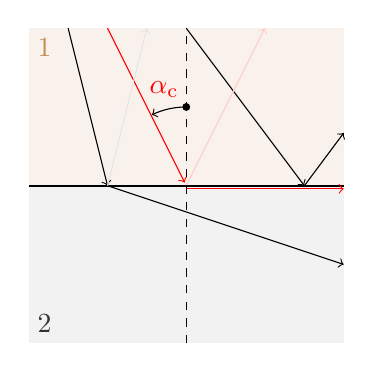
\begin{tikzpicture}
 \fill[brown!10!white] (-2,0) rectangle (2,2);
 \fill[black!5!white] (-2,0) rectangle (2,-2);
 \draw[thick] (-2,0 ) -- (2,0);
 \draw[->, red] (-1,2) -- (-0.02, 0.04);
 \draw[->] (-1.5,2) -- (-1, 0);
 \draw[->] (-1, 0) -- (  2,-1);
 \draw[->] ( 0, 2) -- (1.5, 0);
 \draw[->] (1.5, 0) -- (2, 0.67) ;
 \draw[->, black!10!white] (-1, 0) -- (-0.5,2);
 \draw[->, red!20!white] (0,0) -- (1, 2);
 \draw[->, red] (0,-0.04) -- (2,-0.04);
 \draw[dashed] (0,-2) -- (0,2);
 \draw[->] (0, 1) arc [start angle=90, end angle=116, radius=1];
 \draw[red] (103:1.25) node {$\alpha_\mathrm{c}$};
 \fill (0, 1) circle [radius=0.05];
 \draw[brown!90!white] (-1.8, 1.75) node {$1$};
 \draw[black!80!white] (-1.8,-1.75) node {$2$};
\end{tikzpicture}

\begin{equation*}
 \sin\alpha_\mathrm{c}=\frac{c_1}{c_2} %(P,S)
\end{equation*}

\end{column}
\begin{column}[t]{.675\linewidth}
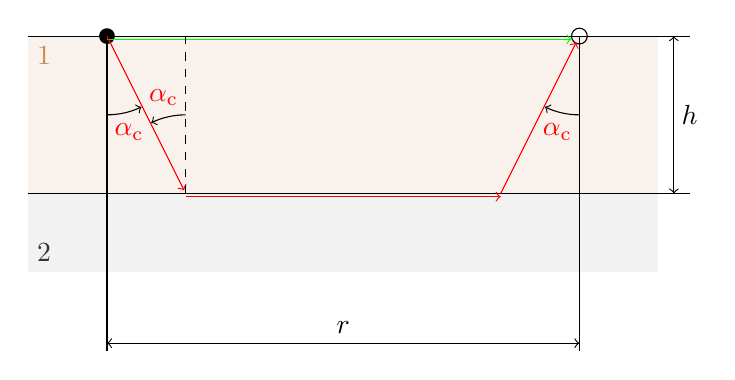
\begin{tikzpicture}
 \fill[brown!10!white] (-2,0) rectangle (6,2);
 \fill[black!5!white] (-2,0) rectangle (6,-1);
 \fill (-1, 2) circle [radius=0.1];
 \draw ( 5, 2) circle [radius=0.1];
 \draw (-1, 2) -- (-1,-2);
 \draw ( 5, 2) -- ( 5,-2);
 \draw[<->] (-1, -1.9) -- ( 5,-1.9);
 \draw (2,-1.7) node {$r$};
 \draw (-2,2 ) -- (6.4,2);
 \draw (-2,0 ) -- (6.4,0);
 \draw[<->] (6.2,0 ) -- (6.2, 2);
 \draw (6.4, 1) node {$h$};
 \draw[->, green] (-1,1.96) -- (4.9, 1.96);
 \draw[->, red] (-1,2) -- (-0.02, 0.04);
 \draw[->, red] (0,-0.04) -- (4,-0.04);
 \draw[->, red] (4, 0) -- ( 4.96, 1.92);
 \draw[dashed] (0,0) -- (0,2);
 \draw[->] ( 0, 1) arc [start angle=90, end angle=116, radius=1];
 \draw[->] (-1, 1) arc [start angle=270, end angle=296, radius=1];
 \draw[red] (103:1.25) node {$\alpha_\mathrm{c}$};
 \draw[red] (-1,2) +(283:1.25) node {$\alpha_\mathrm{c}$};
 \draw[red] ( 5,2) +(257:1.25) node {$\alpha_\mathrm{c}$};
 \draw[->] (5, 1) arc [start angle=270, end angle=244, radius=1];
 \draw[brown!90!white] (-1.8, 1.75) node {$1$};
 \draw[black!80!white] (-1.8,-0.75) node {$2$};
\end{tikzpicture}

\begin{align*}
 {\color{green} t_A} &= \frac{r}{c_1} \\
 {\color{red} t_B} &= \frac{2h}{c_1 \cos\alpha_\mathrm{c}} + \frac{r-2h\tan\alpha_\mathrm{c}}{c_2}
\end{align*}
\end{column}
\end{columns}
}% only

\only<2>{
\begin{columns}
        \begin{column}[t]{.5\linewidth}
        \begin{figure}
%\includegraphics[width=0.95\textwidth]{fig_img/refraction_runtime.png}
\documentclass{article}
\usepackage{tikz}


\begin{document}
    \begin{tikzpicture}[]
        
        %Diagramm
        \draw[->, thick] (0,0) -- (0, 6) node[rotate = 90] at (-0.35, 4) {Laufzeit $[ms]$};
        \draw[->, thick] (0,0) -- (10,0) node[below] {$r[m]$};

        \draw[black, thick, domain = 0:5] plot (\x,  \x) ;
        \draw[black, thick, loosely dashed, domain = 0:2] plot (\x, {0.25*\x + 1.5});
        \draw[black, thick, domain = 2:8] plot (\x, {0.25*\x + 1.5});
        \draw[black, thick, dashed] (2,0) -- (2,2);


    \end{tikzpicture}
\end{document}


\caption*{Laufzeitdiagramm \cite{Schmidt2017}}
        \end{figure}
Voraussetzung $c_2>c_1$

\end{column}
\begin{column}[t]{.5\linewidth}
Abstand $r_c$ gleicher Laufzeit
\begin{align*}
t_A &= t_B \\
 \frac{r_c}{c_1}  &= \frac{2h}{c_1 \cos\alpha_\mathrm{c}} + \frac{r_c-2h\tan\alpha_\mathrm{c}}{c_2} \\
  &= \frac{2h}{c_1 \cos\alpha_\mathrm{c}} + \frac{r_c-2h\tan\alpha_\mathrm{c}}{c_1/\sin\alpha_\mathrm{c}} \\
 &= \frac{2h}{c_1 \cos\alpha_\mathrm{c}} 
 + \frac{r_c\sin\alpha_\mathrm{c}}{c_1}
 - \frac{2h\sin^2\alpha_\mathrm{c}}{c_1 \cos\alpha_\mathrm{c}}  
\end{align*}
Zwischenergebnis
\begin{equation*}
r_c(1-\sin\alpha_\mathrm{c})=2h\frac{1-\sin^2\alpha_\mathrm{c}}{ \cos\alpha_\mathrm{c}}
\end{equation*}

\end{column}
\end{columns}
}% only

\only<3>{
\begin{align*}
 r_c(1-\sin\alpha_\mathrm{c}) &= 2h\frac{1-\sin^2\alpha_\mathrm{c}}{ \cos\alpha_\mathrm{c}} \\
 r_c(1-\sin\alpha_\mathrm{c}) &= 2h\cos\alpha_\mathrm{c}\\
 h &= \frac{r_c(1-\sin\alpha_\mathrm{c})}{2\cos\alpha_\mathrm{c}} 
\end{align*}
Erinnerung an den kritischen Winkel $\sin\alpha_\mathrm{c}=\frac{c_1}{c_2}$
\begin{align*}
 h &=  \frac{r_c(1-c_1/c_2)}{2\sqrt{1-(c_1/c_2)^2}}
 = \frac{r_c(c_2-c_1)}{2\sqrt{c_2^2-c_1^2}} 
 = \frac{r_c(c_2-c_1)}{2\sqrt{(c_2-c_1)(c_2+c_1)}} \\
 h &=\frac{r_c}{2}\sqrt{\frac{c_2-c_1}{c_2+c_1}}   \\ 
\end{align*}
}% only

\only<4
>{
Erweiterungen: 
\begin{itemize}
 \item aus Messung in entgegengesetzter Richtung lässt sich der Neigungswinkel der Bodenschicht bestimmen,
 \item auch für mehr als zwei Schichten anwendbar.
\end{itemize}
Grenzen:
\begin{itemize}
 \item die tieferen Schichten müssen höheren Wellengeschwindigkeiten aufweisen ($c_2>c_1$),
 \item bei P-Wellen stellt der Grundwasserspiegel eine Schichtgrenze dar,
 \item bei größeren Messentfernungen ist der schnellste Wellenweg gekrümmt (tiefenabhängiger E-Modul).
\end{itemize}
}%only

\end{frame}


\begin{frame}
\frametitle{Bohrlochmessungen}

\only<1>{
\begin{figure}
 \includegraphics[width=0.71\textwidth]{fig_img/cross_hole.png}
 \caption*{Cross-hole Messung \cite{Schmidt2017}}
\end{figure}
}%only


\only<2>{
\begin{figure}
 \includegraphics[width=0.71\textwidth]{fig_img/down_hole.png}
 \caption*{Down-hole Messung \cite{Schmidt2017}}
\end{figure}
}%only

\only<3>{
\begin{figure}
 \includegraphics[width=0.71\textwidth]{fig_img/up_hole.png}
 \caption*{Up-hole Messung \cite{Schmidt2017}}
\end{figure}
}%only


\end{frame}


\begin{frame}
\frametitle{R-Wellen Dispersionsmessung}

\only<1>{
\begin{figure}
 \includegraphics[width=\textwidth]{fig_img/rayleigh_measure_principle.png}
 \caption*{\cite{Vrettos2017}}
\end{figure}
Einfache Inversionsregel: Die Rayleigh-Wellengeschwindigkeit entspricht den Bodeneigenschaften in einer Tiefe $z=-\frac{\lambda_\mathrm{R}}{2}$.
}%only

\only<2>{
 \includegraphics[width=0.9\textwidth]{fig_img/rayleigh_measure_velocity.png} \cite{Vrettos2017}
}%only

\only<3>{
\begin{itemize}
 \item Besonders aussagekräftig um die Schwingungsübertragung eines Geländes zu charakterisieren, 
 \item Materialdämpfung kann mit ermittelt werden,
 \item weitgehend unabhängig vom Grundwasserspiegel.
 \item Nachteile: Platzbedarf, starke Schwingungsquelle nötig und nicht geeignet um dünne Schichten zu identifizieren.
\end{itemize}

}%only

\end{frame}

% laboratory measurements
\subsection{Laborversuche}


\begin{frame}
\frametitle{Triaxialversuch}

\begin{figure}
\includegraphics[width=0.82\textwidth]{fig_img/triaxial_test.png}
\cite{Schmidt2017}
\end{figure}
%anisotrope Spannungszustände 
% Einfluss der Belastungsamplitude, Zyklenzahl
% große Verformungen, kleine Frequenzen
\end{frame}


\begin{frame}
\frametitle{Schwingversuche}

\begin{figure}
\includegraphics[width=0.91\textwidth]{fig_img/resonant_column.png}
\cite{Vrettos2017}
\end{figure}

Eigenfrequenz $\leadsto$ Schubmodul, Frequenzgang oder Ausschwingen $\leadsto$ Dämpfung, \textsl{siehe Übung}.
\end{frame}


\begin{frame}
\frametitle{Weitere Verfahren}
\begin{itemize}
 \item Scherversuche 

        \includegraphics[width=0.84\textwidth]{fig_img/shear_test.png} \cite{Vrettos2017}
 
 \item Ultraschallmessung, ähnlich zu Bohrlochmessungen im Gelände
\end{itemize}



\end{frame}


%%%%%%%%%%%%%%%%%%%%%%%%%%%%%%%%%%%%%%%%%%%%%%%%

\section*{Literaturverzeichnis}

\begin{frame}[allowframebreaks]{}
	\printbibliography
\end{frame}
\end{document}
